%!TEX program = xelatex
\documentclass[10pt]{article}
\usepackage{amsthm}
\usepackage{amssymb}
\usepackage{amsmath}
\usepackage{mathrsfs}
\usepackage{titlesec}
\usepackage{xcolor}
\usepackage{enumerate}
\usepackage{bm}
\usepackage{tikz}
\usepackage{listings}
\usetikzlibrary{arrows}
\usepackage{subfigure}
\usepackage{graphicx,booktabs,multirow}
\usepackage[a4paper]{geometry}
\usepackage{upquote}
\usepackage{float}
\usepackage{pdfpages}

\geometry{verbose,tmargin=2cm,bmargin=2cm,lmargin=2cm,rmargin=2cm}
\geometry{verbose,tmargin=2cm,bmargin=2cm,lmargin=2cm,rmargin=2cm}
\lstset{language=Matlab}
\lstset{breaklines}

\input defs.tex

\newtheorem{proposition}{Proposition}
\newtheorem{remark}{Remark}

\titleformat*{\section}{\centering\LARGE\scshape}
\renewcommand{\thesection}{\Roman{section}}
\lstset{language=Matlab,tabsize=4,frame=shadowbox,basicstyle=\footnotesize,
keywordstyle=\color{blue!90}\bfseries,breaklines=true,commentstyle=\color[RGB]{50,50,50},stringstyle=\ttfamily,numbers=left,numberstyle=\tiny,
  numberstyle={\color[RGB]{192,92,92}\tiny},backgroundcolor=\color[RGB]{245,245,244},inputpath=code}

\begin{document}

\date{\today}
\title{Introduction to Machine Learning, Fall 2023 \\
	Homework 2\\
	\small (Due Tuesday Nov. 14 at 11:59pm (CST))}
\maketitle

\begin{enumerate}[1.]


	\item \defpoints{10} [Convex Optimization Basics]
	      \begin{itemize}
		      \item[(a)] Proof any norm $f:\mathbb{R}^{n}\rightarrow\mathbb{R}$ is convex.~\defpoints{2}
		      \item[(b)] Determine the convexity (i.e., convex, concave or neither) of $f(x_1,x_2)=x_1^2/x_2$ on $\mathbb{R}\times\mathbb{R}_{>0}$.~\defpoints{2}
		      \item[(c)] Determine the convexity of $f(x_1,x_2)=x_1/x_2$ on $\mathbb{R}_{>0}^{2}$.~\defpoints{2}
			  \item[(d)] Recall Jensen's inequality $f(\mathbb{E}(X)) \leq \mathbb{E}(f(X))$ if $f$ is convex for any random variable $X$. 
			  Proof the log sum inequality: 
			  \[
				\sum_{i=1}^{n} a_i \log \frac{a_i}{b_i} \geq \left( \sum_{i=1}^{n} a_i\right) \log \frac{\sum_{i=1}^{n} a_i}{\sum_{i=1}^{n} b_i} 
			  \]
			  where $a_1,\ldots,a_n$ and $b_1,\ldots,b_n$ are positive numbers. Hints: $f(x)=x\log x$ is strictly convex.~\defpoints{4}
	      \end{itemize}

		  \textbf{Solution:}

 		  (a) Since $f$ is a norm function, we have the properties of norm functions that,\\
		  1. $\forall \mathbf{x},\mathbf{y}\in \mathbb{R}^{n}, f(\mathbf{x}+\mathbf{y})\leq f(\mathbf{x})+f(\mathbf{y})$.\\
		  2. $\forall \mathbf{x}\in \mathbb{R}^{n}, \forall a \in \mathbb{R}, f(a\mathbf{x})=|a|f(\mathbf{x})$.\\

		  So we have, $\forall \mathbf{x},\mathbf{y}\in \mathbb{R}^{n}, \forall \lambda \in [0,1]$.\\
		  From property 1., we can get that 
		  $$f(\lambda \mathbf{x}+(1-\lambda)\mathbf{y})\leq f(\lambda \mathbf{x})+f((1-\lambda)\mathbf{y})$$
		  From property 2., we can get that
		  $$f(\lambda \mathbf{x})=|\lambda|f(\mathbf{x})\ and\ f((1-\lambda)\mathbf{y})=|1-\lambda|f(\mathbf{y})$$
		  Since $\lambda \in [0,1]$, so we have $|\lambda|=\lambda$ and $|1-\lambda|=1-\lambda$,\\
		  So we can get that
		  $$f(\lambda \mathbf{x}+(1-\lambda)\mathbf{y})\leq \lambda f(\mathbf{x})+(1-\lambda)f(\mathbf{y})$$
		  
		  So above all, from the defination, we can get that $f$ is a convex function.\\

		  (b) Since $f(x_1,x_2)=\dfrac{x_1^2}{x_2}$, so we have the Hessain matrix of $f$ is
		  $$H=\nabla^2f(x_1,x_2)=
		  \begin{bmatrix}
		  \frac{2}{x_2} & -\frac{2x_1}{x_2^2}\\
		  -\frac{2x_1}{x_2^2} & \frac{2x_1^2}{x_2^3}
	      \end{bmatrix}$$
		  Since $x_2 > 0$, so $|H|=\dfrac{2}{x_2}\cdot\dfrac{2x_1^2}{x_2^3}-(-\dfrac{2x_1}{x_2^2})^2=\dfrac{4x_1^2}{x_2^4}-\dfrac{4x_1^2}{x_2^4}=0\geq 0$\\
		  So we can get that $\nabla^2f(x_1,x_2)\succeq 0$, so $f$ is a convex function.\\

		  So above all, $f$ is a convex function.\\

		  (c) Since $f(x_1,x_2)=\dfrac{x_1}{x_2}$, so we have the Hessain matrix of $f$ is
		  $$H=\nabla^2f(x_1,x_2)=
		  \begin{bmatrix}
		  0 & -\frac{1}{x_2^2}\\
		  -\frac{1}{x_2^2} & \frac{2x_1}{x_2^3}
	      \end{bmatrix}$$
		  Since $x_2 > 0$, so $|H|=\dfrac{2x_1}{x_2^3}\cdot 0-(-\dfrac{1}{x_2^2})^2=-\dfrac{1}{x_2^4}\leq 0$\\
		  So we can get that $\nabla^2f(x_1,x_2)\preceq 0$, so $f$ is a concave function.\\

		  So above all, $f$ is a concave function.\\

		  (d) We can construct a distribution $X$ s.t.\\
		  the domain of $X$ is $\dfrac{a_i}{b_i}, i\in\{1,2,\cdots,n\}$, and the PMF of $X$ is $P(X=\dfrac{a_i}{b_1})=\dfrac{b_i}{\sum\limits_{i=1}^{n}b_i}$.\\
		  Since $\forall i \in\{1,2,\cdots,n\}, a_i > 0, b_i > 0$,\\
		  So $P(X=\dfrac{a_i}{b_i}) > 0$, and $\sum\limits_{i=1}^{n}P(X=\dfrac{a_i}{b_i})=1$.\\
		  So it's a valid distribution.\\
		  So $$\mathbb{E}(X)=\sum\limits_{i=1}^{n} (\dfrac{a_i}{b_i})\cdot P(X=\dfrac{a_i}{b_i})=\sum\limits_{i=1}^{n} \dfrac{a_i}{b_i}\cdot \dfrac{b_i}{\sum\limits_{k=1}^{n}b_k}=\dfrac{\sum\limits_{i=1}^{n}a_i}{\sum\limits_{i=1}^{n}b_i}$$

		  And since $f(x)=x\log x$ is strictly convex, so from the Jensen's inequality, we can get that\\
		  $$f(\mathbb{E}(X)) \leq \mathbb{E}(f(X))$$
		  i.e.
		  $$\left(\dfrac{\sum\limits_{i=1}^{n}a_i}{\sum\limits_{i=1}^{n}b_i}\right)\log \left(\dfrac{\sum\limits_{i=1}^{n}a_i}{\sum\limits_{i=1}^{n}b_i}\right) 
		  \leq \sum\limits_{i=1}^{n} P(X=\dfrac{a_i}{b_i})\cdot f(\dfrac{a_i}{b_i})$$
		  $$\left(\dfrac{\sum\limits_{i=1}^{n}a_i}{\sum\limits_{i=1}^{n}b_i}\right)\log \left(\dfrac{\sum\limits_{i=1}^{n}a_i}{\sum\limits_{i=1}^{n}b_i}\right)
		  \leq \sum\limits_{i=1}^{n} \dfrac{b_i}{\sum\limits_{k=1}^nb_k}\cdot(\dfrac{a_i}{b_i})\log(\dfrac{a_i}{b_i})$$
		  
		  Since $b_i>0$, so $\sum\limits_{i=1}^nb_i>0$, so appointment $\sum\limits_{i=1}^nb_i$ on both sides simultaneously, we can get that
		  $$\left(\sum\limits_{i=1}^{n} a_i\right) \log \left(\dfrac{\sum\limits_{i=1}^{n} a_i}{\sum\limits_{i=1}^{n} b_i}\right)
		  \leq \sum\limits_{i=1}^{n} a_i\log \left(\dfrac{a_i}{b_i}\right)$$
		  
		  i.e. $$\sum\limits_{i=1}^{n} a_i \log \frac{a_i}{b_i} \geq \left( \sum_{i=1}^{n} a_i\right) \log \frac{\sum_{i=1}^{n} a_i}{\sum_{i=1}^{n} b_i}$$

		  So above all, with such construction, we have proved the inequality
		  $$\sum_{i=1}^{n} a_i \log \frac{a_i}{b_i} \geq \left( \sum_{i=1}^{n} a_i\right) \log \frac{\sum_{i=1}^{n} a_i}{\sum_{i=1}^{n} b_i}$$

	      \newpage

	\item \defpoints{10} [Linear Methods for Classification] 
	Consider the ``Multi-class Logistic Regression'' algorithm. Given training set 
	$\mathcal{D}=\{(x^i,y^i)\mid i=1,\ldots,n\}$ where $x^i\in \mathbb{R}^{p+1}$ is the 
	feature vector and $y^i\in \mathbb{R}^{k}$ is a one-hot binary vector indicating 
	$k$ classes. We want to find the parameter $\hat{\beta}=[\hat{\beta}_1,\ldots,\hat{\beta}_k]\in \mathbb{R}^{(p+1)\times k}$ 
	that maximize the likelihood for the training set. Introducing the softmax 
	function, we assume our model has the form 
	\[
		p(y_c^i=1\mid x^i;\beta) = \frac{\exp(\beta_c^\top x^i)}{\sum_{c'}\exp(\beta_{c'}^\top x^i)},
	\]
	where $y_c^i$ is the $c$-th element of $y^i$.
		  \begin{itemize}
			\item[(a)] Complete the derivation of the conditional log likelihood for our model, which is
			\begin{align*}
				\ell(\beta) = \ln \prod_{i=1}^{n} p(y_t^i\mid x^i;\beta)
				=\sum_{i=1}^{n}\sum_{c=1}^{k}\left[ y_c^i(\beta_c^\top x^i) - y_c^i\ln \left(\sum_{c'}\exp(\beta_{c'}^\top x^i) \right)\right].
			\end{align*}
			For simplicity, we abbreviate $p(y_t^i=1\mid x^i;\beta)$ as $p(y_t^i\mid x^i;\beta)$, where 
			$t$ is the true class for $x^i$.~\defpoints{4}
			\item[(b)] Derive the gradient of $\ell(\beta)$ w.r.t. $\beta_1$, i.e., 
			\[
				\nabla_{\beta_1}\ell(\beta) = \nabla_{\beta_1} \sum_{i=1}^{n}\sum_{c=1}^{k}\left[ y_c^i(\beta_c^\top x^i) - y_c^i\ln \left(\sum_{c'}\exp(\beta_{c'}^\top x^i) \right)\right].
			\]
			Remark: Log likelihood is always concave; thus, we can optimize our model 
			using gradient ascent. (The gradient of $\ell(\beta)$ w.r.t. $\beta_2,\ldots,\beta_k$ is similar, you don't need to write them)~\defpoints{6}
		  \end{itemize}
		  \textbf{Solution:}\\
		  (a) 






		  (b)







	      \newpage

	\item \defpoints{10} [Probability and Estimation]
	Suppose $\mathcal{D}=\{ x_{1}, x_{2}, \ldots, x_{n} \}$ are i.i.d. samples from exponential distribution with parameter 
	$\lambda > 0$, i.e., $X \sim \text{Expo}(\lambda)$. Recall the PDF of exponential distribution is
	\[
		p(x\mid \lambda) = \begin{cases}
		\lambda e^{-\lambda x},&\quad x > 0 \\
		0,&\quad \text{otherwise}
		\end{cases}.
	\]
	      \begin{itemize}
			\item[(a)] To derive the posterior distribution of $\lambda$, we assume its prior 
			distribution follows gamma distribution with parameters $\alpha,\beta > 0$, i.e., 
			$\lambda \sim\text{Gamma}(\alpha,\beta)$ (since the range of gamma distribution 
			is also $(0,+\infty)$, thus it's a plausible assumption). The PDF of $\lambda$ is 
			given by
			\[
				p(\lambda\mid \alpha,\beta) = \frac{\beta^{\alpha}}{\Gamma(\alpha)} \lambda^{\alpha-1}e^{-\lambda\beta},
			\]
			where $\Gamma(\alpha) = \int_{0}^{+\infty} t^{\alpha-1}e^{-t}dt,\ \alpha>0$. 
			Show that the posterior distribution $p(\lambda\mid \mathcal{D})$ is also a 
			gamma distribution and identify its parameters. Hints: Feel free to drop 
			constants. \defpoints{4}

			\item[(b)] Derive the maximum a posterior (MAP) estimation for $\lambda$ 
			under $\text{Gamma}(\alpha,\beta)$ prior. \defpoints{3}
			
			\item[(c)] For exponential distribution $\text{Expo}(\lambda)$, $\sum_{i=1}^{n} x_{i}\sim \text{Gamma}(n,\lambda)$ 
			and the inverse sample mean $\frac{n}{\sum_{i=1}^{n} x_{i}}$ is the MLE for $\lambda$. 
			Argue that whether $\frac{n-1}{n}\hat{\lambda}_{MLE}$ is unbiased ($\mathbb{E}(\frac{n-1}{n}\hat{\lambda}_{MLE})=\lambda$). 
			Hints: $\Gamma(z+1)=z\Gamma(z)$, $z > 0$. \defpoints{3}
	      \end{itemize}

      	  \textbf{Solution:}\\
		  (a) From Bayes' Rule, we can get that
		  $$p(\lambda|\mathcal{D})=\dfrac{p(\mathcal{D}|\lambda)p(\lambda)}{p(\mathcal{D})}$$
		  Since $\mathcal{D}$ do not contain any $\lambda$, so we can get that
		  $$p(\lambda|\mathcal{D})\propto p(\mathcal{D}|\lambda)p(\lambda)$$
		  And since $\mathcal{D}=\{x_1,x_2,\cdots,x_n\}$ are i.i.d. samples from exponential distribution with parameter $\lambda > 0$, so we can get that
		  $$p(\mathcal{D}|\lambda)=p(x_1,x_2,\cdots,x_n|\lambda)=\prod\limits_{i=1}^np(x_i|\lambda)$$
		  Since $p(x|\lambda)=\lambda e^{-\lambda x},x>0$, so WLOG, we can assume that all the sampling points are positive,
		  i.e. $\forall i, x_i>0$, then we can get that
		  $$p(\mathcal{D}|\lambda)=\prod\limits_{i=1}^n\lambda e^{-\lambda x_i}=\lambda^n e^{-\lambda\sum\limits_{i=1}^nx_i}$$
		  And since we know that the prior distribution of $\lambda$ is that $\lambda\sim Gamma(\alpha,\beta)$,
		  so we can get that
		  $$p(\lambda)=p(\lambda|\alpha,\beta)=\dfrac{\beta^{\alpha}}{\Gamma(\alpha)} \lambda^{\alpha-1}e^{-\lambda\beta}$$
		  So
		  $$p(\lambda|\mathcal{D})\propto \lambda^n e^{-\lambda\sum\limits_{i=1}^nx_i}\cdot\dfrac{\beta^{\alpha}}{\Gamma(\alpha)} \lambda^{\alpha-1}e^{-\lambda\beta}\propto\lambda^{n+\alpha-1}e^{-\lambda(\sum\limits_{i=1}^nx_i+\beta)}$$
		  Since $p(\lambda|\mathcal{D})$ is in terms of conditional probability, so its distribution must be a valid distribution.\\
		  And from $$p(\lambda|\mathcal{D})\propto\lambda^{n+\alpha-1}e^{-\lambda(\sum\limits_{i=1}^nx_i+\beta)}$$
		  we can get that the distribution is $$p(\lambda|\mathcal{D})\sim Gamma(\alpha+n,\beta+\sum\limits_{i=1}^nx_i)$$

		  So above all, we have proved that the posterior distribution $p(\lambda|\mathcal{D})$ is also a Gamma distribution, 
		  and the parameters is that $p(\lambda|\mathcal{D})\sim Gamma(\alpha+n,\beta+\sum\limits_{i=1}^nx_i)$

		  (b) From (a), we get that $p(\lambda|\mathcal{D})\sim Gamma(\alpha+n,\beta+\sum\limits_{i=1}^nx_i)$.\\
		  and $p(\lambda|\mathcal{D})\propto\lambda^{n+\alpha-1}e^{-\lambda(\sum\limits_{i=1}^nx_i+\beta)}$.\\
		  So the MAP for $\lambda$ under $Gamma(\alpha,\beta)$ prior is that
		  $$\hat{\lambda}_{MAP}=\argmax\limits_{\lambda}\lambda^{\alpha+n-1}e^{-\lambda(\beta+\sum\limits_{i=1}^nx_i)}$$
		  Take it into the log-likelyhood function, the result of MAP is the same.\\
		  So
		  $$\hat{\lambda}_{MAP}=\argmax\limits_{\lambda}(\alpha+n-1)\log\lambda-(\beta+\sum\limits_{i=1}^nx_i)\lambda$$
		  Let $$f(\lambda)=(\alpha+n-1)\log\lambda-(\beta+\sum\limits_{i=1}^nx_i)\lambda$$
		  then $$f'(\lambda)=\dfrac{\alpha+n-1}{\lambda}-(\beta+\sum\limits_{i=1}^nx_i)$$
		  And $$f''(\lambda)=-(\alpha+n-1)\dfrac{1}{\lambda^2}<0$$
		  So we could find that the function $f(\lambda)$ is a concave function.\\
		  So to get the MAP, we need to find the point where the first derivative of $f(\lambda)$ is equal to 0.\\
		  i.e. $$\dfrac{\alpha+n-1}{\lambda}-(\beta+\sum\limits_{i=1}^nx_i)=0$$
		  So $$\hat{\lambda}_{MAP}=\dfrac{\alpha+n-1}{\beta+\sum\limits_{i=1}^nx_i}$$

		  So above all, the MAP estimation for $\lambda$ under $Gamma(\alpha,\beta)$ prior is that
		  $$\hat{\lambda}_{MAP}=\dfrac{\alpha+n-1}{\beta+\sum\limits_{i=1}^nx_i}$$

		  (c) Since the MLE is that $\hat{\lambda}_{MLE}=\dfrac{n}{\sum\limits_{i=1}^nx_i}$, so we can get that
		  $$\mathbb{E}(\dfrac{n-1}{n}\hat{\lambda}_{MLE})=\mathbb{E}(\dfrac{n-1}{n}\cdot\dfrac{n}{\sum\limits_{i=1}^nx_i})=\mathbb{E}(\dfrac{n-1}{\sum\limits_{i=1}^nx_i})$$
		  Let $Y=\sum\limits_{i=1}^nx_i$, then $Y\sim Gamma(n,\lambda)$, so we can get that
		  $$\mathbb{E}(\dfrac{n-1}{n}\hat{\lambda}_{MLE})=(n-1)\mathbb{E}(\dfrac{1}{Y})$$
		  Since $Y\sim Gamma(n,\lambda)$, so with LOTUS, we can get that
		  $$\mathbb{E}(\dfrac{1}{Y})=\int_{0}^{+\infty}\dfrac{1}{y}\cdot\dfrac{\lambda^n}{\Gamma(n)}y^{n-1}e^{-\lambda y}dy$$
		  Since $\Gamma(n)=(n-1)\Gamma(n-1)$, so we can get that
		  $$\mathbb{E}(\dfrac{1}{Y})=\int_{0}^{+\infty}\dfrac{\lambda\cdot\lambda^{n-1}}{(n-1)\Gamma(n-1)}y^{n-2}e^{-\lambda y}dy$$
		  $$=\dfrac{\lambda}{n-1}\int_{0}^{+\infty}\dfrac{\lambda^{n-1}}{\Gamma(n-1)}y^{n-2}e^{-\lambda y}dy$$
      	  Since $\dfrac{\lambda^{n-1}}{\Gamma(n-1)}y^{n-2}e^{-\lambda y}$ is the PDF of $Gamma(n-1,\lambda)$,
		  so $$\int_{0}^{+\infty}\dfrac{\lambda^{n-1}}{\Gamma(n-1)}y^{n-2}e^{-\lambda y}dy=1$$
		  so $$\mathbb{E}(\dfrac{1}{Y})=\dfrac{\lambda}{n-1}$$
		  so $$\mathbb{E}(\dfrac{n-1}{n}\hat{\lambda}_{MLE})=(n-1)\mathbb{E}(\dfrac{1}{Y})=(n-1)\cdot\dfrac{\lambda}{n-1}=\lambda$$

		  But there has a problem that, when $n=1$, then in the upper steps, many steps include $\dfrac{1}{n-1}$ become valid, and 
		  $\Gamma(n-1)=\Gamma(0)$ is not valid, $Gamma(n-1,\lambda)\sim\Gamma(0,\lambda)$ is also not a valid distribution.\\
		  Actually, since $\lambda>0$, and when $n=1$, $\mathbb{E}(\frac{n-1}{n}\hat{\lambda}_{MLE})=0\neq\lambda$.\\
		  
		  So above all, when $n=1$, $\dfrac{n-1}{n}\hat{\lambda}_{MLE}$ is not unbiased.\\
		  When $n>1$, $\dfrac{n-1}{n}\hat{\lambda}_{MLE}$ is unbiased.\\

      	  \newpage

	\item \defpoints{10} [Graphical Models]
	Given the following Bayesian Network, 
	\begin{figure}[h]
		\label{fig:bn}
		\vskip 0.2in
		\begin{center}
		\centerline{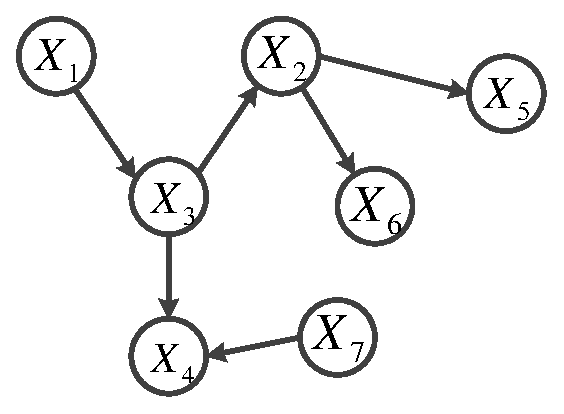
\includegraphics[width=0.4\columnwidth]{figures/bn}}
		%\caption{}
		\end{center}
		\vskip -0.2in
	\end{figure}

	answer the following questions.
		\begin{itemize}
			\item[(a)] Factorize the joint distribution of $X_{1},\cdots,X_{7}$ according 
			to the given Bayesian Network.~\defpoints{2} 
			\item[(b)] Justify whether $X_{1}\perp X_{5}\mid X_{2}$?~\defpoints{2} 
			\item[(c)] Justify whether $X_{5}\perp X_{7}\mid X_{3},X_{4}$?~\defpoints{2} 
			\item[(d)] Justify whether $X_{5}\perp X_{7}\mid X_{4}$?~\defpoints{2} 
			\item[(e)] Write down the variables that are in the Markov blanket of $X_{3}$.~\defpoints{2} 
		\end{itemize}

		\textbf{Solution:}\\
		(a) $P(X_1,\cdots,X_)=P(X_1)P(X_2|X_3)P(X_3|X_1)P(X_4|X_3,X_7)P(X_5|X_2)P(X_6|X_2)P(X_7)$\\

		(b)




		(c)



		(d)




		(e)

		



\end{enumerate}

\end{document}